%-*- coding:utf-8 -*-

\title{ALPSチュートリアル \\ 04 -- Python入門}

\begin{document}

\lstset{language={Python2}}

\begin{frame}
  \titlepage
\end{frame}

\section*{Outline}
\begin{frame}
  \tableofcontents
\end{frame}

\section{Pythonの実行}

\subsection*{\redm\whiteb\greenb}
\begin{frame}[t, fragile]
\frametitle{Pythonの実行}
\begin{itemize}
\item ターミナル(LXTerminal)の中でpythonと入力しEnterキーを押すと、Pythonインタプリタが起動する
  \begin{itemize}
  \item 各行を入力しリターンキーを押すと, 入力内容がすぐさま実行される
  \item Python を終了するには Ctrl-D を入力する
  \end{itemize}
\item Interactive Python (ipython)では, 矢印キー(↑)やCtrl-Rで履歴検索, Tabキーで関数名の補完nなど便利な機能が使える
  \begin{itemize}
  \item MateriApps LIVE!のLXTerminalでは, 背景が黒, ipythonのプロンプトが青で表示され見辛くなっている
  \item LXTerminalの「Edit」メニューから「Preferences」を開き, 背景を白, 文字色を黒に設定し直すことを推奨
  \end{itemize}
\item Pythonコマンドをファイルに書き込み, ``python ファイル名''のように実行することでバッチ実行も可
\item 例の中の行頭の\verb+>>>+はPythonの出力するプロンプト. 入力不要
\end{itemize}
\end{frame}

\subsection*{\redm\whiteb\greenb}
\begin{frame}[t, fragile]
\frametitle{IPython Notebookを使った自習 (オプション)}
\begin{itemize}
\item IPython Notebookとは?
  \begin{itemize}
  \item ブラウザ上でドキュメントとPythonコードを編集・保存できる
  \item Matplotlibによる図もドキュメントに埋め込むことが可能
  \item ドキュメント内でPythonコードを直接実行できる
  \item (最近、''Jupiter Notebook''という名前に変更された)
  \end{itemize}
\item IPython Notebookの起動
\begin{lstlisting}
$ cd $HOME/tutorials/notebook/ja
$ ipython notebook
\end{lstlisting}	 
  \begin{itemize}
  \item ブラウザが立ち上がり, notebookの一覧が表示される
  \item 一番下のpythonをクリックして開く
  \item グレーの枠で囲まれた箇所がPythonのコード. 枠内をクリックして「Shift + Enter」でPythonコードが実行される
  \end{itemize}
\end{itemize}
\end{frame}

\section{データ型}

\subsection*{\redm\whiteb\greenb}
\begin{frame}[t, fragile]
\frametitle{基本的なデータ型}
\alert{このセクションでは Python で使われる基本的なデータ型を紹介する. } array は numpy モジュールで定義されている型で, Python がもともと持っ
ている型ではないが, 科学計算では非常に便利な性質を持つので紹介する. 

\begin{table}[hb]
 \begin{tabular}{r|l} 
  \textbf{数値}       & int, (long), float, complex \\
  \textbf{文字列}     & 'hello,python' \\
  \textbf{list}       & a = [1, 2, 3] \\
  \textbf{tuple}      & b = (1, 2, 3) \\
  \textbf{dictionary} & c = \{'apple': 100, 'orange': 200, 'pear': 300\} \\
  \textbf{set}        & set([1, 2, 3]) \\
  \textbf{bool}       & True, False \\
  \textbf{array}      & numpy array([1,2,3]) \\
 \end{tabular}
\end{table}
\end{frame}

\subsection*{\redm\whiteb\greenb}
\begin{frame}[t,fragile]
\frametitle{数値}
整数, 倍精度浮動小数, 複素数の 3 種類ある. 

\begin{itemize}
 \item int, (long)
 \item float は倍精度のみです. 単精度はない. 
 \item complex
       \begin{itemize}
	\item 'j' もしくは 'J' で虚数部を表す 2 + 3j
	\item 実部 real(2+3j) = 2, 虚部 imag(2+3j) = 3  
       \end{itemize}
 \item 以下のようにして, 型変換を行うことが可能. 

       \begin{columns}
	\begin{column}{4cm}
\begin{lstlisting}
>>> a = 1.8
>>> int(a)
1
\end{lstlisting}	 
	\end{column}
	\begin{column}{4cm}
\begin{lstlisting}
>>> a = 3
>>> float(a)
3.0
\end{lstlisting}	 
	\end{column}
       \end{columns}
\end{itemize}
\end{frame}

\subsection*{\redm\whiteb\greenb}
\begin{frame}[t,fragile]
\frametitle{文字列}
\begin{lstlisting}
>>> s = 'ab:cd:ef'   # 文字列の定義
>>> s = s.split(':') # 指定した文字で文字列を分割
>>> print s
['ab', 'cd', 'ef']
>>> '-'.join(s)      # 指定した文字で文字列同士を結合
'ab-cd-ef'
>>> 'a' + 'b' + 'c'  # 文字列を結合
'abc'
\end{lstlisting}

\begin{itemize}
  \item シングルクォート\verb|'|もしくはダブルクォート\verb|"|で囲った文字列で定義. 
  \item 複数行の文字列は \verb|'''|(シングルクォート3つ) もしくは \verb|"""|(ダブルクォート3つ) で囲む.
\end{itemize}
\end{frame}

\subsection*{\redm\whiteb\greenb}
\begin{frame}[t,fragile]
 \frametitle{list, tuple}
 \begin{lstlisting}
  >>>a = [1,2,3,4,5] # list
  >>>a[0]   # インデックスは 0 スタート
  1         # 要素 1 個だけなら返り値はスカラー
  >>>a[2:4] # 2<=,<4 番目のの要素が返される. 
  [3,4]     # 複数の要素なら返り値はリスト. 
  >>>b = (1,2,3,4,5) # tuple
  >>>b[1:]           # ':' の値を省くこともできる
  (2, 3, 4, 5)
 \end{lstlisting}
 \begin{itemize}
  \item ここではリストの要素として数値のみを扱ったが, python オブジェクトなら何でも リストの要素として扱える
 \end{itemize}
\end{frame}

\subsection*{\redm\whitem\greenb}
\begin{frame}[t,fragile]
\frametitle{list のメソッド}
\begin{lstlisting}
>>>a.reverse() # 要素の並びを逆にする
>>>a           # a そのものが変更されるので注意!
[5, 4, 3, 2, 1]
>>>a.pop()  # リストの最後尾の要素を取りのぞく.
1           # 返り値は取りのぞかれた要素
>>>a
[5, 4, 3, 2]
>>>a.sort() # 要素の並び替え
>>>a
[2, 3, 4, 5]
>>>a.sort(reverse=True) # 逆順
>>>a
[5, 4, 3, 2]
\end{lstlisting}
\begin{itemize}
\item ここではリストの要素として数値のみを扱ったが, python オブジェクトなら何でも リストの要素として扱える
\end{itemize}
\end{frame}

\subsection*{\redm\whitem\greenb}
\begin{frame}[t,fragile]
\frametitle{list と tuple の違う点(1)}
\begin{lstlisting}
>>>b = (1)  # これは tuple にならない!(数式の評価順を制御する普通のカッコ)
>>>type(b)
int         # 整数扱いになる
>>>b = (1,) # 要素 1 個の tuple を定義する
>>>type(b)
tuple       # これはちゃんと tuple になっている
>>>a = [1]  # これは list
>>>type(a)
list
\end{lstlisting}
\end{frame}

\subsection*{\redm\whitem\greenb}
\begin{frame}[t,fragile]
\frametitle{list と tuple の違う点(2)}
\begin{lstlisting}
>>>b += (2, 3, 3)  # 要素を付け加えることはできる
>>>b
(1, 2, 3, 3)
>>>b[3] = 5        # 要素を変更することはできない
Traceback (most recent call last):
  File "<stdin>", line 1, in <module>
TypeError: 'tuple' object does not support item assignment
\end{lstlisting}
\begin{itemize}
\item 要素 1 個の場合の扱いが違う
\item tuple の要素の値は変更できない. 
\item tuple は辞書のキーに登録できる. list は不可. 
\end{itemize}
\end{frame}

\subsection*{\redm\whitem\greenb}
\begin{frame}[t,fragile]
\frametitle{list のコピー}
浅いコピーと深いコピーの 2 種類ある
\begin{columns}
\begin{column}{5cm}
\begin{itemize}
\item 浅いコピーではオブジェクトのアドレスをコピーする
\item 深いコピーではオブジェクトの値をコピーする
\end{itemize}
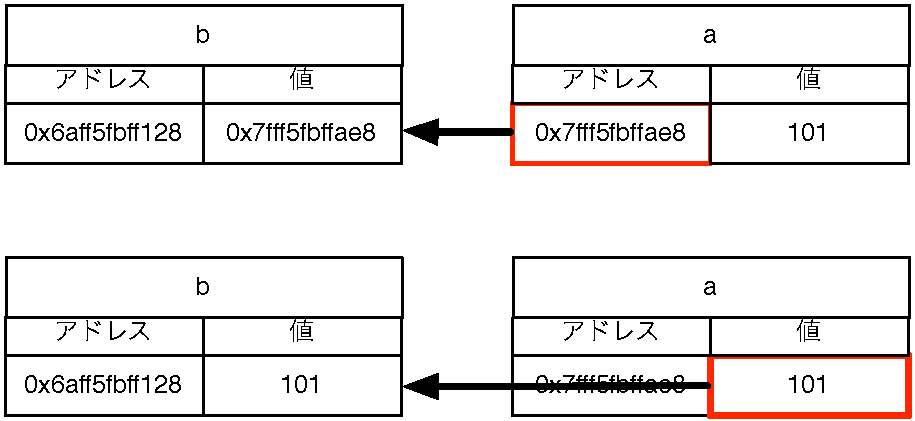
\includegraphics[width = \textwidth]{copy.pdf}
\end{column}

\begin{column}{7cm}
\begin{lstlisting}
>>>a = [101, 102, 103]                 
>>>b = a     # アドレスをコピー
>>>a[1] = 333
>>>print a, b 
[101, 333, 103] [101, 333, 103]
>>>b = a[:]  # 値をコピー
>>>a[1] = 444
>>>print a, b
[101, 444, 103] [101, 333, 103]
\end{lstlisting}
\end{column}
\end{columns}
\end{frame}

\subsection*{\redm\whitem\greenb}
\begin{frame}[t,fragile]
\frametitle{ネストされた list のコピー}
\begin{columns}
\begin{column}{6cm}
浅いコピーになってしまう例
\begin{lstlisting}
>>>a = [1, [2, 3]]
>>>b = a[:]
>>>a[0] = 4
>>>a[1][0] = 5
>>>print a, b
[4, [5, 3]] [1, [5, 3]]
>>>
\end{lstlisting}
\end{column}

\begin{column}{6cm}
深いコピー
\begin{lstlisting}
>>>import copy
>>>a = [1, [2, 3]]
>>>b = copy.deepcopy(a)
>>>a[0] = 101
>>>a[1][0] = 102
>>>print a, b
[101, [102, 3]] [1, [2, 3]]
\end{lstlisting}
\end{column}
\end{columns}

\begin{itemize}
\item ネストされているとスライス ':' で返されるのがアドレスになってしまう
\item ネストされた list で深いコピーをするには copy モジュールの deepcopy を使う
\end{itemize}
\end{frame}

\subsection*{\redm\whiteb\greenb}
\begin{frame}[t,fragile]
\frametitle{辞書型の使い方}
\begin{lstlisting}
>>>dic = {'key0': 0, 'key1': 1}   # key:value の組を登録
>>>dic['key2'] = 2          # key2:2 を登録
>>>dic.keys()               # 辞書に登録されている全ての key
['key2', 'key1', 'key0']
>>>dic.values()             # 全ての val
[2, 1, 0]
>>>dic.items()              # 全ての key:val の組を表示
[('key2', 2), ('key1', 1), ('key0', 0)]  
>>>del dic['key0']          # 辞書から key を削除
>>>dic.items()
[('key2', 2), ('key1', 1)]
\end{lstlisting}

\begin{itemize}
\item 辞書の要素はソートされていない. 登録順なども関係ない. 
\end{itemize}
\end{frame}

\section{制御フロー}

\subsection*{\redm\whitem\greenb}
\begin{frame}[t,fragile]
\frametitle{if-elif-else 文の使い方}
if-elif-else で条件分岐を作れる.
インデントの深さ(文頭の空白の数)でブロックを表現する.
\begin{lstlisting}[stepnumber=1]
>>>if a > 0: # コロン : を忘れずに
>>>    print '0'
>>>elif a == 0:
>>>    print '1'
>>>else:
>>>    print '2'
>>>
>>>
\end{lstlisting}

条件演算子(三項演算子)

\begin{lstlisting}
>>>val = val1 if cond1 else val2
\end{lstlisting}
\end{frame}

\subsection*{\redm\whiteb\greenb}
\begin{frame}[t,fragile]
\frametitle{for 文の使い方}
\verb|in| の後ろにあるシーケンス(リストやタプルなど)の中身を, 先頭から順に\verb|i| へと代入しながら, ブロックを繰り返し実行する.
ブロックはインデントの深さ(文頭の空白の数)で表現する.
\begin{lstlisting}
>>>for i in ('a', 'b', 'c', 'd'): # コロン : を忘れずに
>>>    print i,    # コンマで改行を抑制している
a b c d
\end{lstlisting}

アンパック代入と enumerate()
\begin{lstlisting}
>>>for i,j in enumerate(('a', 'b', 'c', 'd')):
>>>    print i, j
0 a
1 b
...
\end{lstlisting}
アンパック代入は python で使える一般的なテクニック. 
\begin{lstlisting}
>>>i,j,k = ['a', 'b', 'c']
\end{lstlisting}
\end{frame}

\subsection*{\redm\whitem\greenb}
\begin{frame}[t,fragile]
\frametitle{while 文の使い方}
\begin{lstlisting}
a = 0
while a in range(10): # コロン : を忘れずに
    a += 1
    if a < 3:
        continue
    elif a == 8:
        break
    print a

\end{lstlisting}

\begin{itemize}
\item カレントディレクトリに上の内容で exWhile.py というファイルを作って import してみよう.
\item "val in シークエンス:" というフレーズは while だけでなく if, for など至る所で使える.
\item continue, break も同じく if, for などでも使える.
\end{itemize}
\end{frame}

\section{関数}

\subsection*{\redm\whiteb\greenb}
\begin{frame}[t,fragile]
\frametitle{関数}
\begin{lstlisting}
>>> def f(x, y): # コロン : を忘れずに
>>> ....z = x * y  # 空白 4 つのインデント!
>>> ....for i in [1, 2, 3]:
>>> ....    z += i
>>> ....return z
>>>
>>> f(2,3)
12
\end{lstlisting}
\begin{itemize}
\item def 関数名(引数,...): で関数が定義できる
\item Python ではインデント (ここの例では空白4つ) によりスコープを制御する
\end{itemize}
\end{frame}

\section{モジュール(ライブラリ)}

\subsection*{\redm\whiteb\greenb}
\begin{frame}[t]
\frametitle{Python プログラムの階層構造}
\begin{itemize}
\item プログラムファイルのディレクトリ構成 == 名前空間
\item モジュール
\begin{itemize}
 \item 1 つの "hoge.py" ファイルが 1 つのモジュール
\end{itemize}
\item パッケージ
\end{itemize}
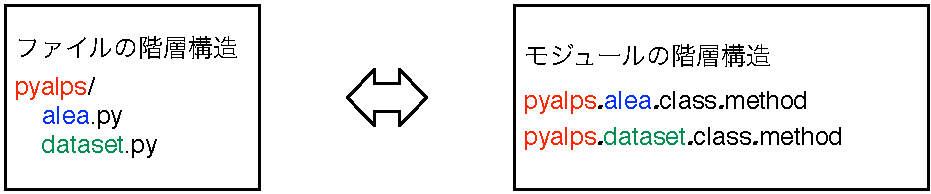
\includegraphics[width=\textwidth]{module.pdf}
\end{frame}

\subsection*{\redm\whiteb\greenb}
\begin{frame}[t,fragile]
\frametitle{モジュールの読み込み}
\begin{lstlisting}
>>> import fff as f    # 別名をつけてインポート
>>> f.ggg(x, y)
...
>>> from fff import *  # fff 以下のすべてをインポート
>>> ggg(x, y)          # 名前空間 fff が外れる
...
>>> from fff import ggg as g # ggg のみを指定してインポート
>>> g(x, y)
\end{lstlisting}
\begin{itemize}
\item fff モジュール中の ggg 関数を呼び出している. 
\item 呼び出し方により名前空間の階層が変わる. 
\end{itemize}
\end{frame}

\section{ファイルの読み書き}

\subsection*{\redm\whitem\greenb}
\begin{frame}[t,fragile]
\frametitle{ファイルの読み書き}
\begin{columns}
\begin{column}{8cm}
ファイルにデータを書き出す方法
\begin{lstlisting}
xs = ['a', 'b', 'c']
ys = [3.432, 1.42, 2.159]
f = open('dat.txt', 'w')
for x,y in zip(xs,ys):
    f.write('{} {}\n'.format(x,y))
f.close()
\end{lstlisting}
\end{column}
\begin{column}{4cm}
出力データ (dat.txt)
\begin{lstlisting}
a 3.432
b 1.42
c 2.159
\end{lstlisting}
\end{column}
\end{columns}

\begin{itemize}
\item open で dat.txt ファイルを書き込みモードで読み込む
\item zip は複数のシーケンスからタプルのシーケンスを作る関数
\item f.write はファイル\verb|f|に文字列を書き込む関数
\item s.format は文字列\verb|s|中の\verb|{}| に引数の値を文字列化したものを埋め込む関数
\end{itemize}
 一般的にはファイルを使い終わったら f.close() で閉じなければならないが,
 \verb|with open('dat.txt') as f:| とすると、ブロックが終わったら自動で閉じてくれる.
\end{frame}

\begin{frame}[t,fragile]
\frametitle{ファイルの読み書き}
\begin{columns}
\begin{column}{8cm}
ファイルから1行ごとにデータを読み込む方法
\begin{lstlisting}
for line in open('dat.txt', 'r'):
    items = line.split('')
    print items[0], float(items[1])
\end{lstlisting}
\end{column}
\begin{column}{4cm}
入力データ (dat.txt)
\begin{lstlisting}
a 3.432
b 1.42
c 2.159
\end{lstlisting}
\end{column}
\end{columns}

\begin{itemize}
\item open で dat.txt ファイルを readonly で読み込む
\item 読み込んだファイルを 1 行毎に処理する. 読み込まれた行は 1 つのス
      トリングとして扱われるので区切り文字(今の場合空白)で分割してい
      る. 
\item 読み込んだストリングを浮動小数点にキャストしている. 
\end{itemize}
  上の例では\verb|with open() as f:| と同様に, for 文の終了とともにファイルは自動で閉じられる. 
\end{frame}

%% \section{環境設定}
%% \begin{frame}[t,fragile]
%% \frametitle{デフォルトの環境設定}
%% 図の中で使われる文字のサイズや, 図の縦・横のサイズなどをあらかじめ設定しておくことができます. 
%% \begin{itemize}
%% \item matplotlib \$\{HOME\}/.matplotlib/matplotlibrc で設定する
%% \begin{itemize}
%% \item テンプレを \$PYTHONHOME/lib/site-packages/matplotlib/mpl-data/matplotlibrc からコピーして使う
%% %% /opt/local//Library/Frameworks/Python.framework/Versions/2.7/lib/python2.7/site-packages/matplotlib/mpl-data/matplotlibrc
%% \item プロット時にウィンドウを開いて図を表示するには, Mac OS X の場合は次のような設定が必要
%%   \begin{lstlisting}
%% #backend : Agg
%% backend : MacOSX
%% \end{lstlisting}
%% \item 逆にウィンドウを開きたくないなら Agg に設定する
%% \item AGG: Anti-Grain Geometry. ベクトルデータを画像に描くライブラリ. C++ 用. 
%% \end{itemize}
%% \end{itemize}

%% \end{frame}

%% \begin{frame}[t,fragile]
%% \frametitle{動的に環境設定を行う}
%% \begin{itemize}
%% \item backend の設定は import matplotlib の直後にすること
%%       \begin{lstlisting}
%% >>> import matplotlib as mpl
%% >>> mpl.use('Agg')
%% \end{lstlisting}
%% \item グラフのサイズやフォントのサイズの設定
%%       \begin{lstlisting}
%% >>> import pylab
%% >>> params = {
%% ...     'legend.fontsize': 10
%% ...     'xtick.labelsize':  8
%% ...     'ytick.labelsize':  8
%% ...     'figure.figsize':  [width, height]}
%% >>> pyalps.rcParams.update(params)
%% \end{lstlisting}
%% \end{itemize}
%% \end{frame}

\section{Matplotlib入門}

\subsection*{\redm\whiteb\greenb}
\begin{frame}[t,fragile]
\frametitle{簡単な図をプロットしてみる}
\begin{columns}
\begin{column}{6cm}
$y = x^2$ のプロット
\begin{lstlisting}
>>> import pylab as pl
>>> x = range(-10,11) # 11 は含まないので注意
>>> y = [i*i for i in x]
# シンボルの色を赤(r), 形を丸(o)に設定
>>> pl.plot(x, y, 'ro')
...[<matplotlib.lines.Line2D at 0x114c82710>]
# 拡張子で保存のファイル形式が決まる
>>> pl.savefig('x2.pdf') 
>>> pl.show()
\end{lstlisting}
\end{column}

\begin{column}{6cm}
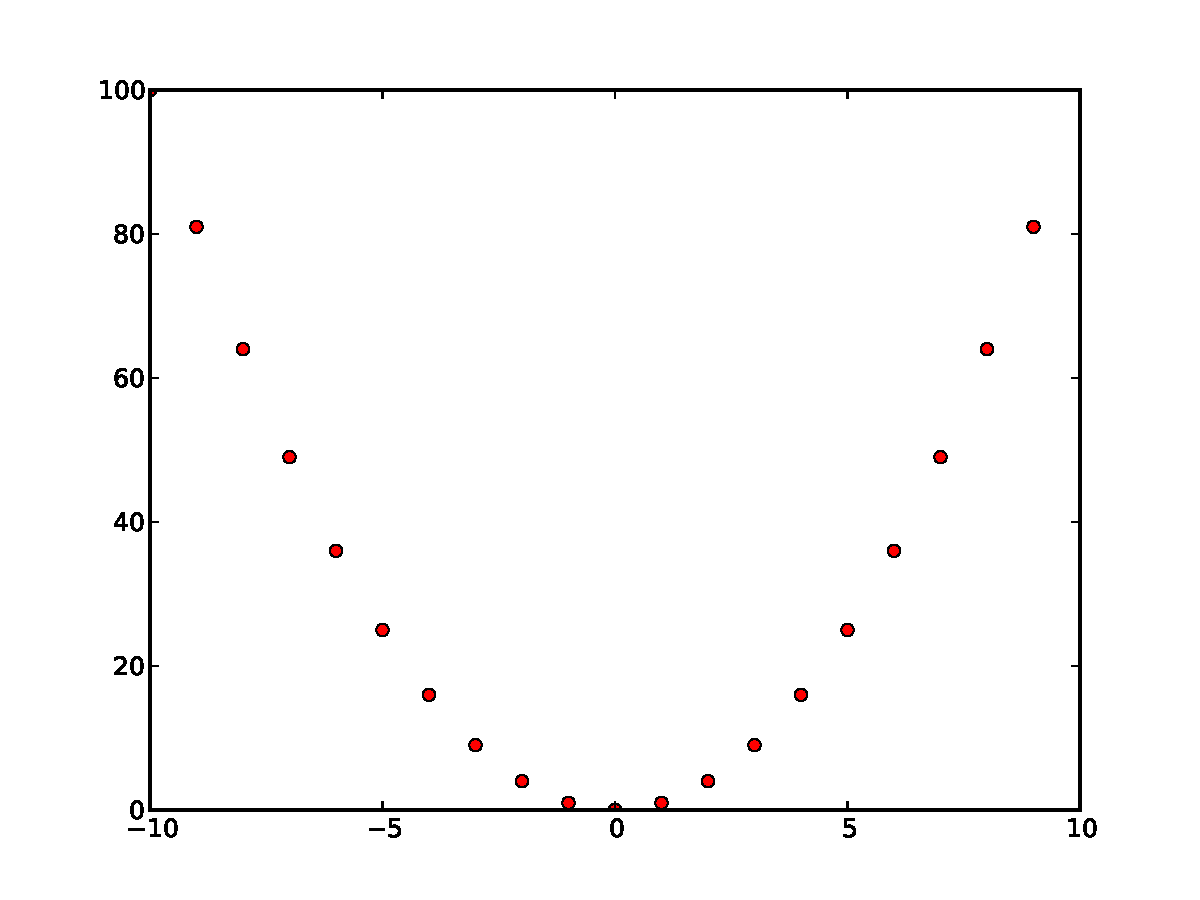
\includegraphics[width=\textwidth]{x2.pdf}
\end{column}
\end{columns}
\verb|ro| に \verb|-| を付け加えるとシンボルが実線で結ばれる.
他のシンボルなどは \verb|pl.plot?| としてヘルプを参照.
\end{frame}

\subsection*{\redm\whitem\greenb}
\begin{frame}[t,fragile]
\frametitle{少し複雑な図をプロットしてみる}
\begin{lstlisting}
>>> import math as m       # cos を使うため
>>> x = range(-10,11)
>>> y1 = [i*i for i in x]
>>> y2 = [i*i*i for i in x]
>>> y3 = [m.cos(2 * m.pi * i/20) for i in x]
# 図を上下 2 段に並べてプロットします
>>> pl.subplot(211)        # 上側の図を書き始める. 2行1列の1つ目.
>>> pl.plot(x, y1, 'ro')   # 1 つのグラフに
>>> pl.plot(x, y2, 'b^')   # 2 つのデータセットをプロット. 青(b)の上向き三角(^)
>>> pl.title('$x^2$ and $x^3$')   # 図のタイトル. TeX も Ok!
>>> pl.legend(('$y1$', '$y2$'), numpoints=1)  # 凡例
\end{lstlisting}
次のページへ続く
\end{frame}

\subsection*{\redm\whitem\greenb}
\begin{frame}[t,fragile]
\frametitle{続き}
\begin{columns}
\begin{column}{6cm}
\begin{lstlisting}
# 下側の図を書き始める.
>>> pl.subplot(212) # 2行1列の2つ目
>>> pl.plot(x, y3, 'gs') # 緑(g) の四角(s)
>>> pl.title('$\cos(x)$')
>>> pl.xlabel('x')
>>> pl.ylabel('y')
>>> pl.savefig('x3.pdf') 
>>> pl.show()
\end{lstlisting}
\end{column}
\begin{column}{6cm}
出来上がり!
\begin{center}
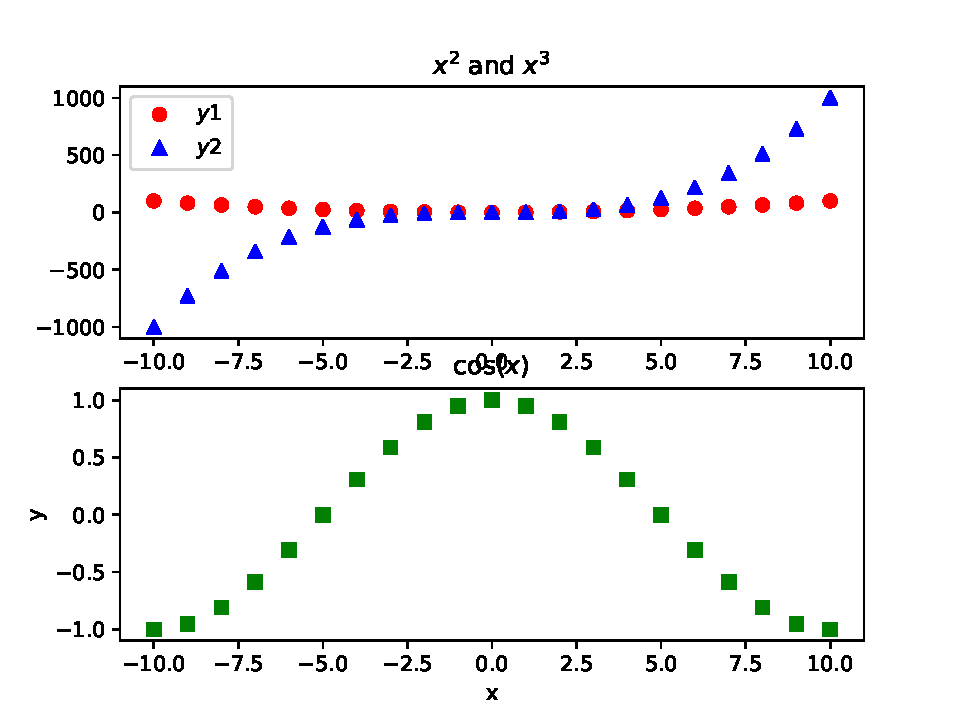
\includegraphics[width=\textwidth]{x3.pdf}
\end{center}
\end{column}
\end{columns}
\end{frame}

\subsection*{\redm\whitem\greenb}
\begin{frame}[t,fragile]
\frametitle{Figure と Axes}
Matplotlib の描画領域には 2 つの座標系がある. 
Figure と Axes です. 1 つの Figure は 1枚の紙で, そこに複数のグラフ (Axes) を描くというイメージ. 

Subplot は Axes の特殊なものです. subplot(col,row,pos) で描画位置を指定できる. 

\begin{center}
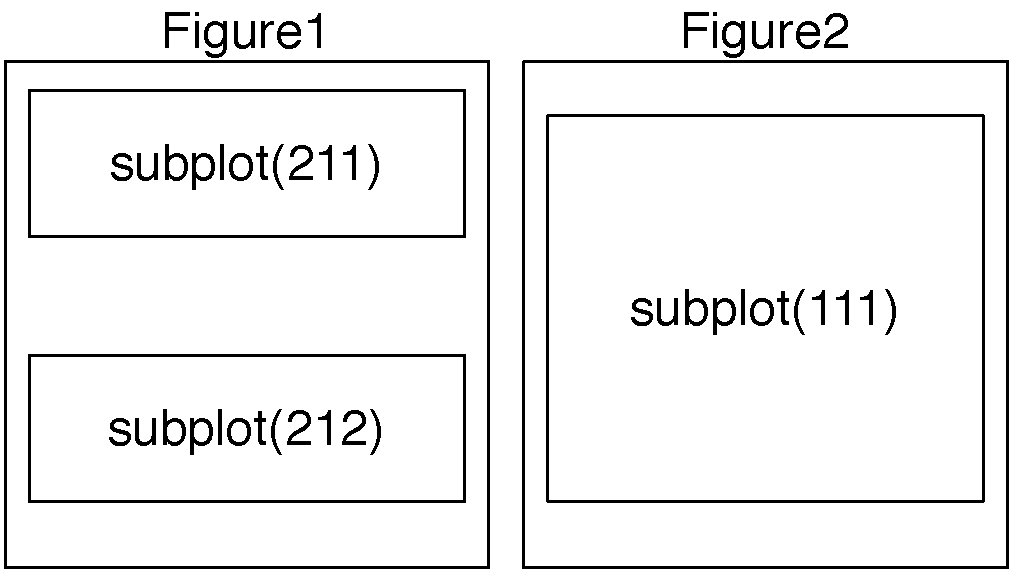
\includegraphics[scale=0.4]{fig_ax.pdf}
\end{center}
\end{frame}

\subsection*{\redm\whitem\greenb}
\begin{frame}[t,fragile]
\frametitle{Current Figure/Axes vs. オブジェクト指向}
今まで紹介してきたプロットは, 暗黙のうちに Current Figure/Axes への操作を行っていた. 複数の Figure を同時に扱いたい場合はオブジェクト指向的なプロット方法が便利.

\begin{columns}
\begin{column}{.52\textwidth}
\begin{lstlisting}
import pylab as pl

pl.figure() 
pl.plot(pl.rand(1000), 'o')

pl.figure()
pl.plot(pl.rand(1000), '^')

pl.show()
\end{lstlisting}
\end{column}

\begin{column}{.52\textwidth}
\begin{lstlisting}
import pylab as pl
fig1 = pl.figure() 
fig2 = pl.figure()

ax1 = fig1.add_subplot(111)  
ax2 = fig2.add_subplot(111)  

ax1.plot(pl.rand(1000), 'o')
ax2.plot(pl.rand(1000), '^')

pl.show()
\end{lstlisting}
\end{column}
\end{columns}
\end{frame}

\section{参考文献}

\subsection*{\redm\whiteb\greenb}
\begin{frame}[t]
\frametitle{参考文献}
\begin{itemize}
\item 科学技術計算のために python を始めよう
  \url{http://www.ike-dyn.ritsumei.ac.jp/~uchida/scipy-lecture-notes/intro/index.html}
\item 初心者のはまりどころ \url{http://webtech-walker.com/archive/2010/10/13191417.html}
\item Doug Hellmannさん \url{http://doughellmann.com}
  \begin{itemize}
  \item 標準モジュールなどの使い方が例とともに書いてあり分かりやすい
  \end{itemize}
\item matplotlib入門 \url{http://yubais.net/doc/matplotlib/}
\item IPython Notebook チュートリアル \url{http://qiita.com/payashim/items/d4fe5227b21a5215e78b}
\end{itemize}
\end{frame}

\end{document}
